\documentclass[12pt,letterpaper,noanswers]{exam}
%\usepackage{color}
\usepackage[usenames,dvipsnames,svgnames,table]{xcolor}
\usepackage[margin=0.9in]{geometry}
\renewcommand{\familydefault}{\sfdefault}
\usepackage{multicol}
\pagestyle{head}
\usepackage{hyperref}
\definecolor{c07}{HTML}{BBFFBB}
\definecolor{c08}{HTML}{BBFFFF}
\definecolor{c09}{HTML}{BBDDFF}
\definecolor{c10}{HTML}{BBBBFF}
\definecolor{c11}{HTML}{DDBBFF}
\definecolor{c12}{HTML}{BBBBDD}
\newcommand{\mb}[1]{\underline{#1}}

\header{AM 22b Problem Set 05}{}{Due Thurs Mar 11 at 6pm ET}
\runningheadrule
\headrule
\usepackage{diagbox}
\usepackage{graphicx} % more modern
%\usepackage{subfigure} 
\usepackage{amsmath} 
\usepackage{amssymb} 
%\usepackage{gensymb} 
%\usepackage{natbib}
\usepackage{hyperref}
%\usepackage{enumitem}
%\setlength{\parindent}{0pt}
%\usepackage{setspace}
%\pagestyle{empty}  
%\newcommand{\Sc}[0]{
%{\color{BlueViolet}\S}
%}
\usepackage{tcolorbox}

\begin{document}
 \pdfpageheight 11in 
  \pdfpagewidth 8.5in

\begin{questions}
\question Log in to WeBWorK and complete the problems assigned there under pset05.


% \question Evaluate the following integrals (show your mathematical work):
% \begin{parts}
% \item \[\int_0^1\int_{e^y}^e \frac{x}{\ln x}\ dx \ dy.\]  \emph{Reversing the order of integration may be helpful.}
% \item \[\int_0^{\pi/6}\int_0^{2/\cos\theta} r\ dr\ d\theta\]  \emph{Convert to Cartesian coordinates.}
% \end{parts}

\question A city surrounds a bay as shown below.  The population density of the city (in thousands of people per square km) is $\delta(r,\theta)$ where $r$ and $\theta$ are polar coordinates and distances are in km.



\begin{parts}
\part Set up an iterated integral in polar coordinates giving the total population of the city.
\part The population density decreases the farther you live from the shoreline of the bay; it also decreases the farther you live from the ocean.  Which of the following functions best describes this situation?  Justify your answer.
\begin{itemize}
\item $\delta(r,\theta) = (4-r)(2+\cos\theta)$
\item $\delta(r,\theta) = (4-r)(2+\sin\theta)$
\item $\delta(r,\theta) = (4+r)(2+\cos\theta)$
\item $\delta(r,\theta) = (4+r)(2+\sin\theta)$
\end{itemize} 
%  \part Estimate the population by combining your answers above, and evaluating.
\end{parts}


 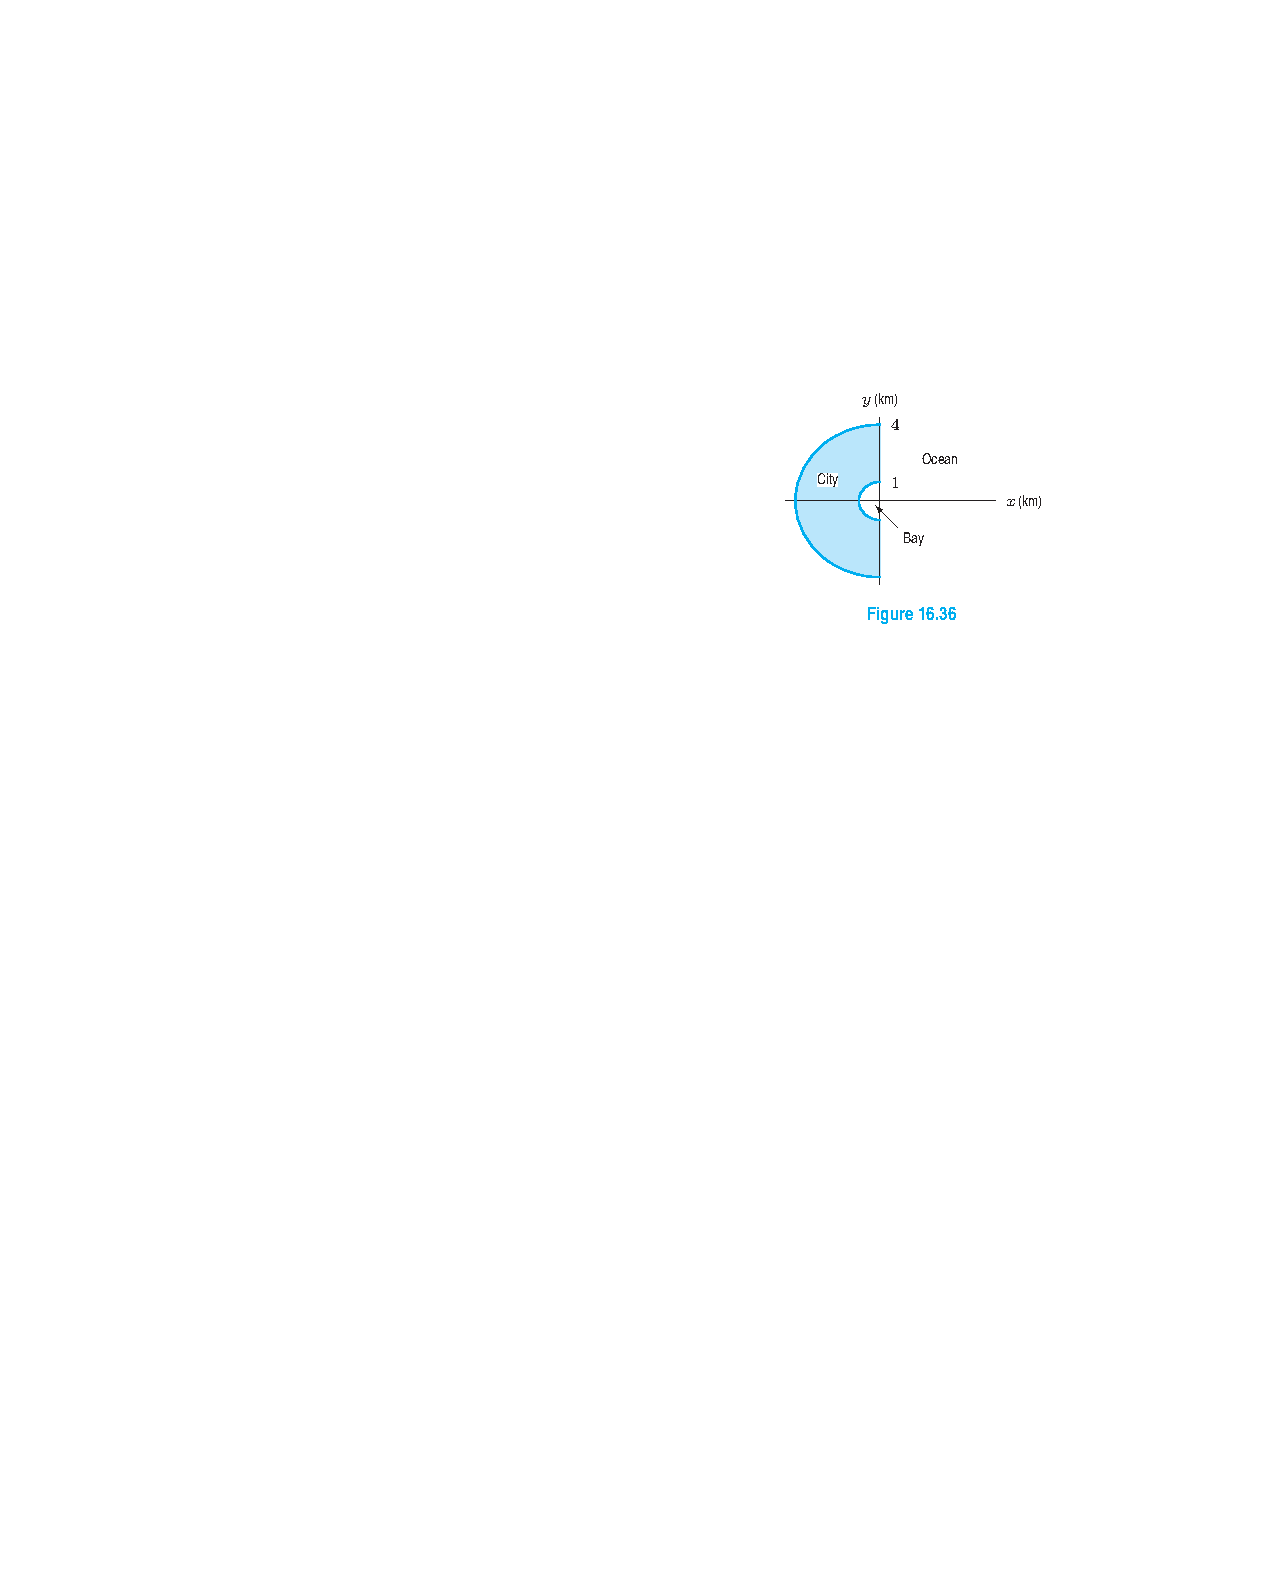
\includegraphics{img/HW07p2.pdf}
 
 \begin{solution}

 The population is given by \[\iint_R \delta(r,\theta) dA = \int_{\pi/2}^{3\pi/2}\int_1^4\delta(r,\theta)\ rdrd\theta.\]

The population decreases as we move away from the shoreline of the bay at $r=1$.  The function $(4-r)$ decreases in this way while $(r+4)$ increases as we move away from the shoreline.  So the function will be (i) or (ii). 

The population decreases as we move away from the ocean at $x = 0$.  

The function $(2+\cos\theta) = 2$ on the half-lines $\theta=\pi/2$, $\theta = 3\pi/2$, and decreases to $1$ as $\theta\rightarrow\pi$.  

The function $(2+\sin\theta)$ is $3$ when $\theta=\pi/2$ and is $1$ when $\theta = 3\pi/2$, while is $2$ in between.  

The $(2+\cos\theta)$ behavior better models decreasing population as we move away from the ocean.  

Thus the function that matches both parts of the description is $\delta(r,\theta) = (4-r)(2+\cos\theta)$.

 \end{solution}

% \question 
% \begin{parts}
% \item 
% Find the area inside the curve $r = 2+ 3\cos\theta$ and outside the circle $r = 2$.  Include a sketch of the region of integration and show your mathematical work.  \emph{To sketch, using WolframAlpha may be helpful:} \texttt{ParametricPlot[\{(2 + 3 Cos[t]) Cos[t], (2 + 3 Cos[t]) Sin[t]\}, \{t, 0, 
%   2 Pi\}]}

% \item Write a triple integral representing the volume of the region between spheres of radius $1$ and $2$, both centered at the origin.  Include limits of integration but do not evaluate.
% \begin{itemize}
% \item Sketch a cross-section of the region in the $rz$-half plane (recall that $r$ is always non-negative).
% \item Use spherical coordinates to write the triple integral.
% \item Use cylindrical coordinates.  \emph{You may wish to write your answer as the difference of two integrals when using cylindrical coordinates.}
% \end{itemize}
% % \end{parts}



% \question Let $W$ be the solid pyramid bounded by the planes $x+z = 6$, $x-z = 0$, $y+z = 6$, $y-z=0$, and above the plane $z = 0$.  The density at any point in the pyramid is given by $\delta(x,y,z) = z$ grams per cm$^3$ where $x,$ $y, $ and $z$ are measured in cm.

% \includegraphics{img/HW07p1.pdf}
% \begin{parts}
% \part What does the triple integral $\int_W z\ dV$ represent?
% \part In evaluating the integral above, consider setting the integral up with the $z$-direction integrated first.  How many separate iterated triple integrals would be needed?
% \part Set up and evaluate an iterated triple integral in a well-chosen order to find $\int_W z\ dV$.
% \end{parts}







\item Write a triple integral that gives the volume above the paraboloid $z=x^2+y^2$ and below sphere $x^2+y^2+z^2=2$. 
\begin{parts}
\item Use Matlab to visualize the region of integration by plotting the two surfaces.  Submit your plot as part of the assignment.

For the sphere, plotting the upper hemisphere will be sufficient.  

Include axis labels on your plot.
\begin{solution}
For the top half of the sphere we have $z = \sqrt{2-x^2-y^2}$ so we need to modify the second function.
\begin{verbatim}
syms x y
domain = [-2 2 -2 2];
fsurf(x,y,x^2+y^2,domain,'facealpha',0.7,'edgecolor','none')
hold on
fsurf(x,y,sqrt(2-x^2-y^2),domain,'facealpha',0.7,'edgecolor','none')
axis equal
xlabel('x'); ylabel('y'); zlabel('z');
set(gca,'fontsize',14)
axis([-1.5 1.5 -1.5 1.5 0 1.5])
caxis([0 2])
\end{verbatim}

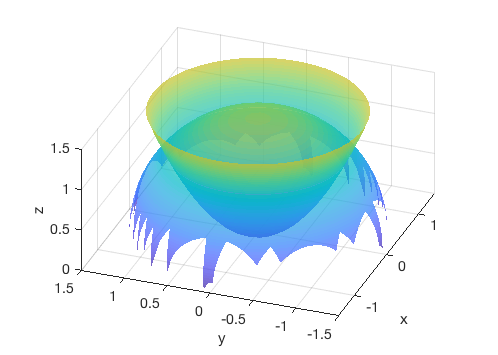
\includegraphics[width=3in]{img/pset07-p1-18.png}
\end{solution}
\item Find an equation describing the $(x,y)$ values of points on the curve of intersection of the two surfaces.
\begin{solution}
We have 
$\left\{\begin{array}{c} z = x^2+y^2 \\ x^2+y^2+z^2 = 2\end{array}\right.$

Substituting $z$ for $x^2+y^2$, this is
$\left\{\begin{array}{c} z = x^2+y^2 \\ z+z^2 = 2\end{array}\right.$

The quadratic $z^2+z-2=0$ factors as $(z-1)(z+2) = 0$ so $z =1$ or $z=-2$.  We know $z>0$ so $z = 1$.

We have
$\left\{\begin{array}{c} 1 = x^2+y^2 \\ z = 1\end{array}\right.$

so $x^2+y^2=1$ is an equation describing the $(x,y)$ values of the points on the curve of intersection.
\end{solution}
\item Setup a triple integral for the volume of the region.
\begin{solution}
We could use any of our three coordinate systems for the setup.  Cylindrical will be nicest, though, because the object is radially symmetric about an axis (we can think of it as being a shape that is spun around an axis).

In Cartesian, this is the region between $z = x^2+y^2$ and below $z = \sqrt{2-x^2-y^2}$ and above the disk $x^2+y^2\leq 1$ in the $xy$-plane.  The disk is being set by where the two surfaces intersect.

A triple integral is adding up $f\Delta V$.  We want to find volume, so we just want to add up $\Delta V$.  $f = 1$.

$\displaystyle \int_{-1}^1\int_{-\sqrt{1-x^2}}^{\sqrt{1-x^2}}\int_{x^2+y^2}^{sqrt{2-x^2-y^2}}1\  dz\ dy\ dx$

I'm not going to want to integrate this in Cartesian (too many square roots). Let's head to cylindrical (the natural coordinate system for the problem because of the radial symmetry about the $z$-axis).

\begin{verbatim}
>> rv = 0:0.01:1;
>> fill([rv, rv(end:-1:1)],[rv.^2,sqrt(2-rv(end:-1:1).^2)],'b')
>> axis equal
>> axis([0 1 0 1.5])
>> set(gca,'fontsize',14)
>> xlabel('r');ylabel('z');
\end{verbatim}

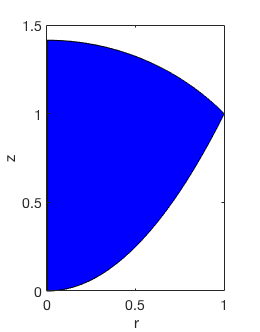
\includegraphics[width=1.5in]{img/pset07-p2-18.png}

In cylindrical, $z = x^2+y^2 = r^2$ and $z = \sqrt{2-x^2-y^2} = \sqrt{2-r^2}$.

$\displaystyle\int_0^{2\pi}\int_0^1\int_{r^2}^{\sqrt{2-r^2}}1\ r\ dz\ dr\ d\theta.$  The $r$ is the Jacobian for cylindrical.

I could set this up in spherical as well.  I would need to use two integrals though.

\begin{verbatim}
rv = 0:0.01:1;
fill([rv, rv(end:-1:1)],[rv,sqrt(2-rv(end:-1:1).^2)],'b')
hold on
fill([rv, rv(end:-1:1)],[rv.^2,rv(end:-1:1)],'r')
axis equal
axis([0 1 0 1.5])
set(gca,'fontsize',14)
xlabel('r');ylabel('z');
\end{verbatim}

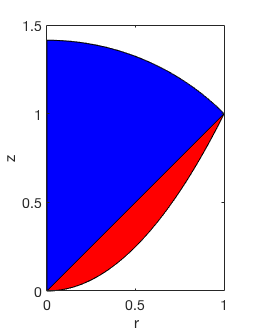
\includegraphics[width=1.5in]{img/pset07-p3-18.png}

The blue part has $\rho$ from $0$ to $\sqrt{2}$ and $\phi$ from $0$ to $\arccos(1/\sqrt{2}).$  The red part has $\rho$ from $0$ to $z = r^2$ so $\rho\cos\phi = \rho^2(\sin\phi)^2$ so $\rho = \frac{\cos\phi}{(\sin\phi)^2}$.
It looks like $\phi$ ranges from $\arccos(1/\sqrt{2})$ to $\pi/2$.

$\displaystyle\int_0^{2\pi}\int_0^{\arccos(1/\sqrt{2})}\int_0^{\sqrt{2}}\rho^2\sin\phi d\rho d\phi d\theta + \int_0^{2\pi}\int_{\arccos(1/\sqrt{2})}^{\pi/2}\int_0^{\cos\phi/(\sin\phi)^2}\rho^2\sin\phi d\rho d\phi d\theta$.  Recall that $\rho^2\sin\phi$ is the Jacobian for spherical coordinates.

\end{solution}
\item Evaluate the integral to find the volume.
\begin{solution}
Cylindrical has the nicest setup.
    
\begin{align*}
\int_0^{2\pi}\int_0^1\int_{r^2}^{\sqrt{2-r^2}}1\ r\ dz\ dr\ d\theta &= \int_0^{2\pi}\int_0^1(\sqrt{2-r^2}-r^2)\ r\ dr\ d\theta \\
&= \int_0^{2\pi}\left.-\frac{1}{3}(2-r^2)^{3/2}-\frac{1}{4}r^4\right\vert_0^1\ d\theta \\
&= \int_0^{2\pi}-\frac{1}{3}(1-2^{3/2})-\frac{1}{4}(1)\ d\theta \\
&= \int_0^{2\pi}2^{3/2}/3-\frac{7}{12}\ d\theta  \\
&= \frac{4\sqrt{2}\pi}{3} -\frac{7\pi}{6}
\end{align*}

Check integrals using matlab:
\begin{verbatim}
int((sqrt(2-r.^2)-r.^2).*r,r)
int((sqrt(2-r.^2)-r.^2).*r,r,0,1)
int(int((sqrt(2-r.^2)-r.^2).*r,r,0,1),th,0,2*pi)
\end{verbatim}
Using matlab I find $(2*2^(1/2))/3 - 7/12$ for the middle integral, which is what I found myself and I find $(pi*(8*2^(1/2) - 7))/6$, which is equivalent to what I found myself.
\end{solution}
\end{parts}


\item Write an iterated integral which represents the mass of a solid ball of radius $a$.  The density at each point in the ball is $k$ times the distance from that point to a fixed plane passing through the center of the ball.  Evaluate the integral.


\question (A connection between $e$ and $\pi$).
A Gaussian function in one variable is a function $f(x) = ke^{-(x-x_0)^2/(2b^2)}$.  

\begin{parts}
\item Plot $f(x) = e^{-x^2/2}$.
\item How does changing $x_0$, $k$, or $b$ change the shape of the function?

\vspace{0.2cm}

 The Gaussian function is the basis of an important probability density function called the \textbf{normal} distribution.   Consider a two-dimensional version, $f(x,y) = k e^{(-x^2-y^2)/2}$.  For this to be a probability density function, we would need $\int_{-\infty}^\infty\int_{-\infty}^\infty f(x,y)\ dx\ dy = 1$.  Find $k$ so that $f(x,y)$ is a probability density function.  We'll tackle this in two different ways: this week we will work analytically and on pset06 we'll use Monte Carlo integration to estimate the value.
\item Find $k$ analytically by integrating $\displaystyle\int_{-\infty}^\infty\int_{-\infty}^\infty e^{(-x^2-y^2)/2}\ dx\ dy$.  Convert to polar to do this integral.

\item Explain why \[\int_{-\infty}^{\infty}\int_{-\infty}^{\infty} e^{-(x^2+y^2)/2}\ dx\ dy = \left(\int_{-\infty}^{\infty}e^{-x^2/2}\ dx\right)^2.\]

\item Find $\displaystyle\int_{-\infty}^{\infty}e^{-x^2/2}\ dx$ and then construct a normal distribution in one variable, where the normal distribution is a probability density function proportional that is proportional to $e^{-x^2/2}$.
\end{parts}


\item Two independent random numbers $x$ and $y$ are each drawn from between $0$ and $1$ with uniform probability.  They have a joint density function of $p(x,y) = 1$ if $0\leq x,y\leq 1$ and $p(x,y) = 0$ otherwise.  We are interested in their sum, $z = x+y$.  

We don't know $x$ and $y$ (they are unknown random numbers), but we have been given their joint probability density function.  It should be possible for us to find a probability density function for $z$.

\begin{parts}
\item We will start with a simulation: 
\begin{itemize}
    \item Generate two random numbers drawn from between $0$ and $1$ (using a uniform probability).
    \item Find their sum.
    \item Store the value of that sum.
    \item Do this 50000 times.
    \item Make a histogram representing the distribution.
\end{itemize} 

\item Still working numerically, convert your histogram to an approximation of the probability density function.
\begin{itemize}
    \item Identify the number of entries in each bin of the histogram.
    \item Compute the proportion of the total number of runs that fell into each bin.
    \item Use the size of each bin to convert from a proportion to an estimate of the probability density function.
\end{itemize}

\item Find the probability density function analytically.


% \begin{lstlisting}
% numberofpoints = 50000;
% data = rand(numberofpoints,2);
% meanvalue = (data(:,1)+data(:,2))/2;

% subplot(1,2,1)
% histogram(meanvalue,'normalization','cdf')
% xlabel('mean value'); ylabel('fraction');
% title({'approximate cumulative', 'distribution function'})
% set(gca,'fontsize',14)
% hold on
% syms x
% fplot(x^2,[0 1],'linewidth',2)
% hold off

% subplot(1,2,2)
% histogram(meanvalue,'normalization','pdf')
% xlabel('mean value'); ylabel('fraction per unit length');
% title({'approximate probability', 'density function'})
% set(gca,'fontsize',14)
% hold on
% fplot(x^3,[0 1],'linewidth',2)
% hold off
% \end{lstlisting}
\end{parts}

%We have probability density information for $x$ and $y$, so  we can find a probability density function for $z$.  To do this, first you'll find the cumulative distribution function, and then you'll find the probability density function.
\begin{itemize}
\item Start by finding the cumulative distribution function for the sum.  Let $F(t)$ be that cdf.  This is a function that returns the probability that the sum, $z$, is less than $t$, where $t$ is the name of the input variable to the function.  %This is called the \textbf{cumulative distribution function} of $z$.
\begin{itemize}
\item Identify values of $t$ where $F(t)$ is either zero or one.  
\item Find $F(t)$ for $0<t\leq 1$.  This is the probability that $0< x+y \leq t$ for $0<t\leq 1$ (so the fraction of the time that $z \leq t$ when $t$ is a number in between $0$ and $1$.) To do this, identify the region in $x,y$-space for which $x+y\leq t$.  $F(t) = \int_S p(x,y)\ dA$, where $S$ is the region in $2$-space where $x+y\leq t$.
\item Use a similar method to find $F(t)$ for $1< t \leq 2$.
\end{itemize}

\begin{solution}
$F(t) = 0$ when $t\leq 0$ since the mean cannot be below $0$ when both $x$ and $y$ are non-negative.  In addition, the mean cannot be greater than $1$ so $F(t) = 1$ for $t\geq 1$.

In between, the fraction of the time $0\leq (x+y)/2\leq t$ is given by the area of the region where $x+y<2t$ and $x\geq 0, y\geq 0$.  

Three cases are shown below, with $t = 0.25, t=0.5,$ and $t=0.75$.

\includegraphics{img/HW07s6.pdf}

For $t\leq 0.5$, $F(t)$ is given by an integral from $y=0$ to $x+y = 2t$ with $x$ ranging from $0$ to $2t$.  The integrand is the probability density for $(x,y)$, which is $1$.
\begin{align*}
F(t) &= \int_0^{2t}\int_0^{2t-x} 1\ dy\ dx \\
&= \int_0^{2t} (2t-x)\ dx \\
&= 4t^2- \int_0^{2t}x\ dx \\
&= 4t^2- \frac{1}{2}(2t)^2 \\
&= \frac{1}{2}(2t)^2 \\
&= 2t^2.
\end{align*}

This is the area of the triangle with base $2t$ and height $2t$.

From $0.5<t<1$, $F(t)$ is given by the area of the region with $0\leq x,y\leq 1$ and $x+y\leq 2t$.  The intersection of $y=1$ and $x+y = 2t$ occurs when $x = 2t-1$.
\begin{align*}
F(t) &=\int_0^{2t-1} \int_0^1 \ dy\ dx + \int_{2t-1}^1\int_0^{2t-x} \ dy\ dx\\
&= 2t-1+\int_{2t-1}^1(2t-x)\ dx \\
&= 2t-1 + 2t(1-(2t-1))- \frac{1}{2}(1-(2t-1)^2) \\
&= 2t-1 + 4t - (2t)^2- \frac{1}{2}(1-(4t^2-4t+1)) \\
&= 6t-1 - (2t)^2- (-2t^2+2t) \\
&= 6t-1 - (2t)^2+2t^2-2t \\
&= 4t-1 - 2t^2 \\
\end{align*}
This should be $1 - (1-(2t-1))^2/2$, the area of the region less the area of the triangle in the corner, which is $-1+4t-2t^2$.

\[ F(t) = \begin{cases} 
      0 & t\leq 0 \\
      2t^2 & 0<t\leq \frac{1}{2} \\
      -1+4t-2t^2 & \frac{1}{2}< t\leq 1 \\
      1 & 1< t 
   \end{cases}
\]


\end{solution}


\item The probability that $z \leq t$ is given by $\int_{-\infty}^t f(z)\ dz$ where $f(z)$ is the probability density function for $z$.  Find $f(z)$.
\item Identify the point with highest density.
\begin{solution}
We have $F(t) = F(0)$ for $t\leq 0$ so we have $\int_0^t f(s)\ ds = F(t) - F(0)$.  By the fundamental theorem of calculus, $f(t) = \frac{dF}{dt}$.

$F(t)$ is a piecewise function so $f(t)$ will be as well.  Taking the derivatives, we find

\[ f(t) = \begin{cases} 
      0 & t\leq 0 \\
      4t & 0<t\leq \frac{1}{2} \\
      4-4t & \frac{1}{2}< t\leq 1 \\
      0 & 1< t 
   \end{cases}
\]

Plotting this, the probability density function for the mean of the two numbers is:

\includegraphics[width=3in]{img/HW07s7.pdf}

The most likely value is where $f(t)$ is maximum, so that value is $0.5$.
\end{solution}

% \part Check your work by generating approximations of the cumulative distribution function and of the probability density function using matlab.  Plot your $F(t)$ in place of $x^2$ to compare it to the numerically generated distribution function.  Plot your $f(t)$ in place of $x^3$ to compare it to the numerically generated density function.  Submit your plots as part of your assignment.
% \begin{verbatim}
% numberofpoints = 50000;
% data = rand(numberofpoints,2);
% meanvalue = (data(:,1)+data(:,2))/2;

% subplot(1,2,1)
% histogram(meanvalue,'normalization','cdf')
% xlabel('mean value'); ylabel('fraction');
% title({'approximate cumulative', 'distribution function'})
% set(gca,'fontsize',14)
% hold on
% syms x
% fplot(x^2,[0 1],'linewidth',2)
% hold off

% subplot(1,2,2)
% histogram(meanvalue,'normalization','pdf')
% xlabel('mean value'); ylabel('fraction per unit length');
% title({'approximate probability', 'density function'})
% set(gca,'fontsize',14)
% hold on
% fplot(x^3,[0 1],'linewidth',2)
% hold off
% \end{verbatim}

\begin{solution}
\begin{verbatim}
numberofpoints = 50000;
data = rand(numberofpoints,2);
meanvalue = (data(:,1)+data(:,2))/2;
subplot(1,2,1)
histogram(meanvalue,'normalization','cdf')
xlabel('mean value'); ylabel('fraction');
title({'approximate cumulative', 'distribution function'})
set(gca,'fontsize',14)
hold on
syms t
fplot(2*t^2,[0 1/2],'linewidth',2)
fplot(-1+4*t-2*t^2,[1/2 1],'linewidth',2)
hold off
subplot(1,2,2)
histogram(meanvalue,'normalization','pdf')
xlabel('mean value'); ylabel('fraction per unit length');
title({'approximate probability', 'density function'})
set(gca,'fontsize',14)
hold on
fplot(4*t,[0 1/2],'linewidth',2)
fplot(4*(1-t),[1/2 1],'linewidth',2)
hold off
\end{verbatim}
\includegraphics[width=\linewidth]{img/pset08p1.png}
\end{solution}
\end{itemize}



\end{questions}

\end{document}
